\chapter{Identifying the Environment Model }
\begin{itemize}
	\item What is the importance of model identification?
    \item How to identify?
    \item What's the data availability and quality?
    \item Are there differences for identifying different kind of models?
    \item What are the challenges?
\end{itemize}
Physiological models are developed to represent certain physiological condition in general, or the physiological condition of a specific patient. Therefore the structure of the model and corresponding parameters have to be identified. These information can be obtained from physiological data, which are from: 1) data collected during physiological procedures, and/or 2) physiological literature in which physiological data are analyzed and summarized. Due to limitation on the interactions with the patient, the availability and quality of physiological data are generally bad and there are not enough information to identify all the parameters in the model. It is essential to choose the right level of abstraction so that the model is identifiable (to a large extend). Having physiological correspondence for the model structure and parameters can also simplify the identification process. The rigorousness of the model identification step is also an important factor for the validity of the model. 

In the following sections, we briefly discuss our model identification effort for heart models used in two closed-loop verification applications, and their corresponding challenges. 

\section{Heart Model Identification for Closed-loop Simulation}
In closed-loop simulation, a heart model should be identified to represent a specific patient under certain heart condition. The constraints for model parameters can be obtained from patient data during \emph{ElectroPhysiological (EP) Testing}. During EP testing, the physicians deliver electrical pacing sequence from electrodes placed inside the patient's heart while extracting timing parameters from observed pattern and timing of electrical events. Since the goal for any EP testing procedure is not to determine all the timing parameters for a patient, the amount of parameters that can be identified from the patient data is limited.    

\figref{modelID} illustrates how timing parameters can be extracted during an EP testing procedure. Assume that there are two electrodes placed in the right atrium and right ventricle of the heart respectively (\figref{modelID}.a), and EGM signals can be measured (\figref{modelID}.b). The physician can also apply pacing sequences through the electrodes which can trigger different response from the patient's heart. \figref{modelID}.c shows a heart model structure with unknown parameter values, which can be extracted by analyzing the \emph{timing} and \emph{pattern} of the local activations. 
\begin{figure}[!t]
\centering
		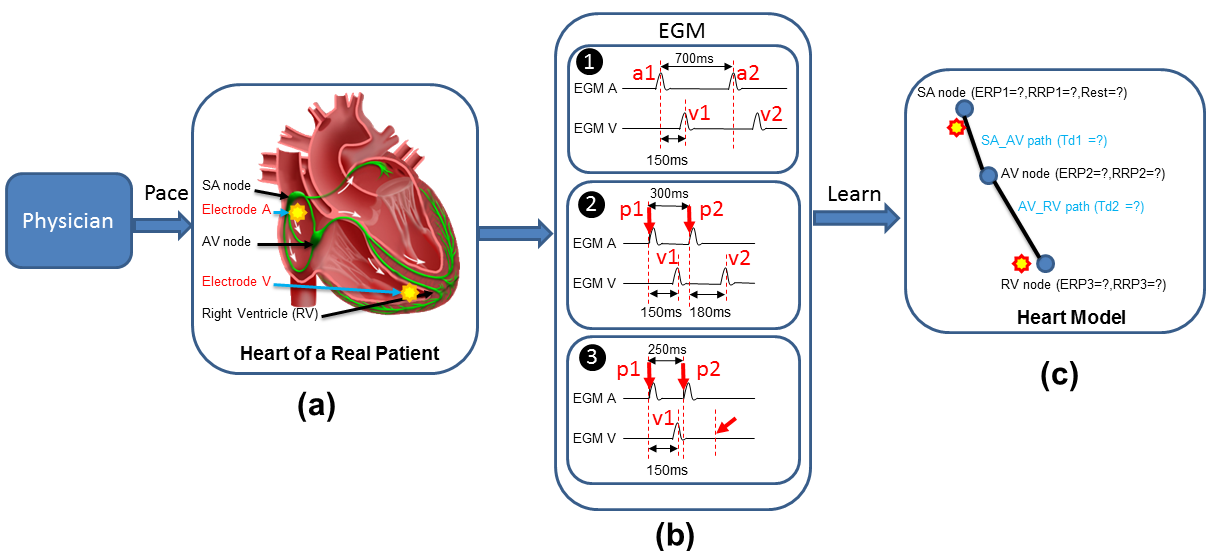
\includegraphics[width=0.9  \textwidth]{figs/modelID.png}
		
%\vspace{-10pt}
\caption{\small (a) Node automaton. Dotted transition is only valid for pacemaker tissue like SA node; (b) Path automaton; (c) Model of the electrical conduction system of the heart using a network of node \& path automata~\cite{vhm_ecrts10}.}
\label{fig:modelID}
%\vspace{-15pt}
\end{figure} 


\section{Heart Model Identification in Closed-loop Model Checking}
In model checking, the heart models in general have simple structure and less parameters due to non-deterministic abstraction. The heart models are developed in consistent with Electrophysiology terminologies, thus each node and path automata and their timing parameters have physiological correspondence which can be found in literature (\cite{josephson}). The range for non-deterministic parameters directly correspond to the range for possible values of corresponding physiological parameters. Therefore model identification for model checking is much simpler. 

An example: \Hao{Need a photo of table of typical parameter values}







\chapter{Validating the Environment Model}
\begin{itemize}
	\item What are the different methods to validate physiological models?
    \item How much confidence can these validation provide?
\end{itemize}
The validity of the environment models affects the validity of the closed-loop verification results. Since models are always approximations of the actual environment, there is always discrepancies between the model and the actual patient (group). The challenge then is to determine how much safety guarantee that model-based closed-loop verification can provide. 

\section{Validate deterministic models}
For deterministic models there are two applications: 1) model a patient with certain heart condition, 2) model a \emph{specific} patient with certain heart condition. For the first application, it is important to show that the model successfully models the underlying mechanism of the heart condition, while for the second application the model should be able to generate same data as the corresponding patient given the same input. 

\subsection{Validating the underlying mechanism}


\begin{figure*}[!t]
\centering
		\subfigure 	[\small Testing result for a real patient (~\cite{josephson})] 
		{
		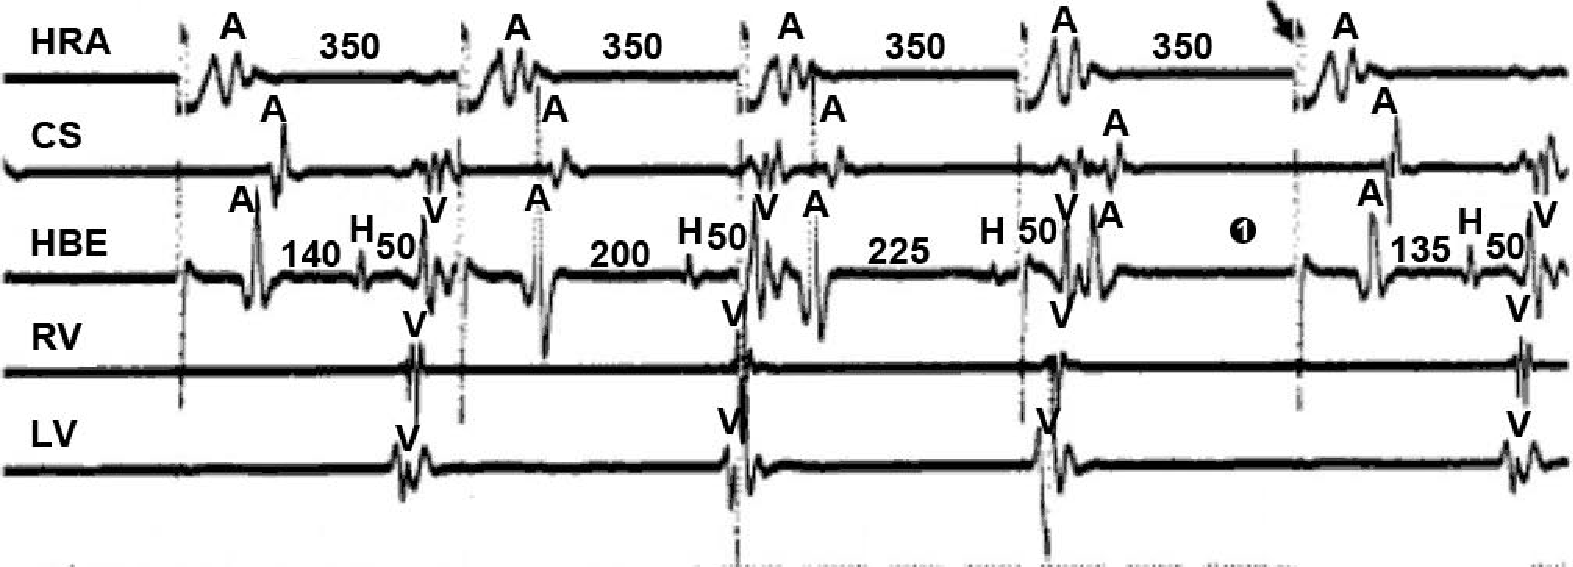
\includegraphics[width=0.45\textwidth]{figs/WB_book.pdf}
		\label{fig:book_1}
		} 
		\subfigure [\small Testing result for VHM simulation] 
		{	
			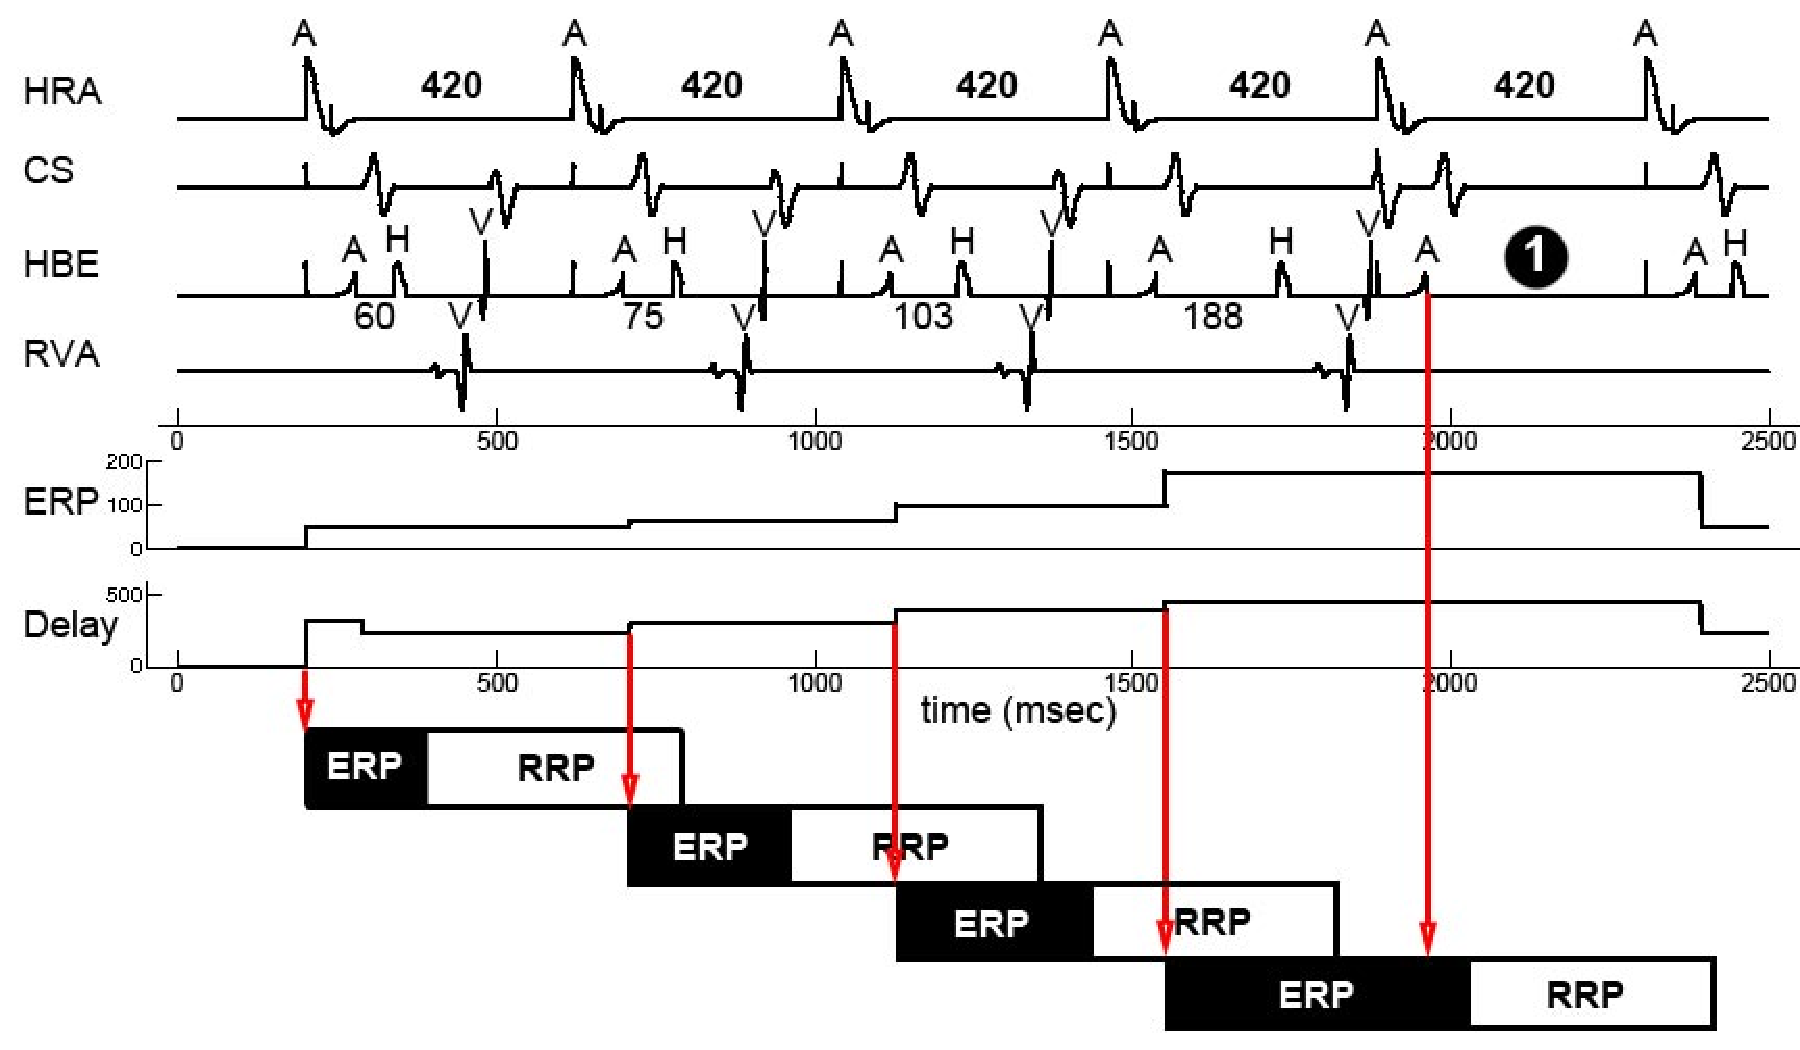
\includegraphics[width=0.40\textwidth]{figs/WB_new.pdf} 
			\label{fig:type_1}
		}
\label{fig:Case_1}
%\vspace{-5pt}
\caption{\small Key interval values when the coupling interval shortens for (a) a real patient and (b) in VHM simulation ~\cite{vhm_ecrts10}.}
%\vspace{-15pt}
\end{figure*} 

\subsection{Validating the accuracy of model identification}

% \begin{figure}[\b]
% 	\center
% 	\vspace{-20pt}
% %	\includegraphics[width=0.49\textwidth]{figs/AV_reentry_circuit.pdf}
% 	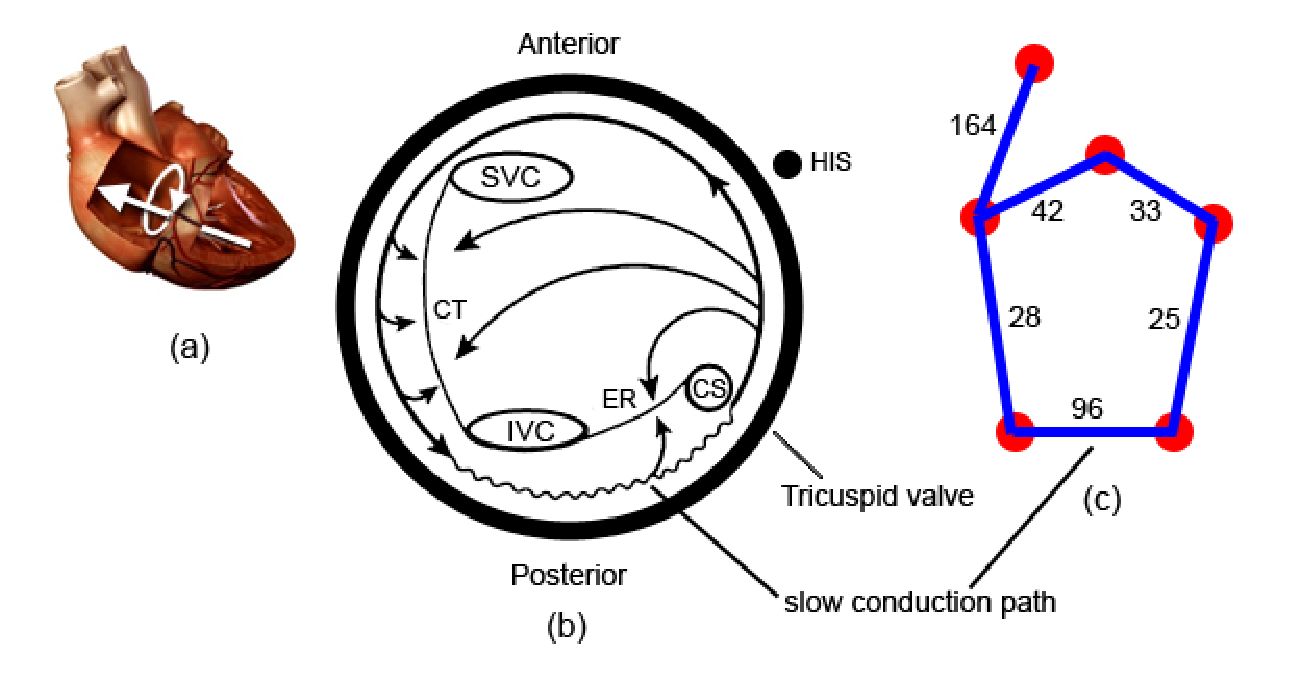
\includegraphics[width=0.5\textwidth]{figs/AFL_circuit.pdf}
% 	\center
% 	\vspace{-15pt}
% 	\caption{(a) The straight arrow shows the view of the AFL circuit from the right ventricle through the tricuspid valve into the right atrium, while the curved area shows the direction of conduction. (b) The circuit is bounded by the eustachian ridge (ER), connecting the  inferior vena cava (IVC) and the coronary sinus (CS), as well as the crista terminalis (CT), connecting the superior vena cava (SVC) and the IVC. The wavy line shows slow conduction through the CTI, bounded by the ER and the tricuspid valve (\emph{Adapted from} \cite{AFL_diag}). (c) The AFL circuit in the VHM extrapolates nodes and paths from the true physiology. The numbers show the values of conduction timers in the paths, with corresponding slow conduction path on the bottom.}
% 	\label{fig:AFL}
% \end{figure}

\section{Validate by Translating Domain Knowledge**}
For non-deterministic models
\begin{itemize}
	\item The physiological basis for the initial model come from literature
    \item All the abstraction rules follow literature
    \item Models before and after the abstraction have simulation relationships
    \item Ranges of parameters come from literature.
\end{itemize}

 